%!TEX root = main.tex
%\paragraph{$R_0$ definition}
%
The basic reproductive number, which is generally denoted by $ R_0 $,
is a threshold quantity with which we can use 
particular control strategies. The epidemiological interpretation of 
$ R_0 $ is the average number of secondary cases produced by an infected
individual introduced into a population of susceptible individuals.
Using Van DenDrishe's \cite{VandenDriessche2017a} definition of reproductive number
we obtain
\begin{equation*}
    \label{eqn:reproductive_number}
    \begin{aligned}
        R_0 :=
        &
        \frac{\kappa}{(\kappa + \mu)(\delta_L + \mu)}
        \left(
           \mu R_1 + \delta_L
        \right)
        \left[
            \frac{p\beta_S}{R_2}
            +\frac{(1 - p) \beta_A}{\gamma_A+\mu}
        \right],
    \\
    \text{where} &
    \\
        R_1 &= 1 - \theta(1 - \epsilon),
    \\
        R_2 &= \mu + \delta_H + \gamma_S + \mu_{I_{S}}.
    \end{aligned}
\end{equation*}
%
Factor $\frac{p\beta_S}{R_2}$ measures the proportion of new infections
generated by a symptomatic infectious individual in the time that it lasts
infected. Similarly, factor $\frac{(1 - p) \beta_A}{\gamma_A+\mu}$
measures the new infections generated by an asymptomatic infectious individual
Term  
$
    \frac{\mu R_1 + \delta_L}{\delta_L + \mu}
$ measures the number of individuals in lockdown that leave the 
lockdown, which can be infected.
And $\frac{\kappa}{\kappa + \mu}$ acount
the incubation period.
%
If we consider that there is no lockdown, then  $ R_0 $ results
\begin{equation*}
    \label{eqn:reproductive_number}
    \begin{aligned}
        \tilde{R}_0 :=
        &
        \frac{\kappa}{(\kappa + \mu)}
        \left[
            \frac{p\beta_S}{R_2}
            +\frac{(1 - p) \beta_A}{\gamma_A+\mu}
        \right].
    \end{aligned}
\end{equation*}
%
Note that we have the relation $ R_0 \leq \tilde{R}_0 $. These indicate that there is greater transmission of the disease if there is no lockdown.
\comment[id=SDIV]{%
    Here countor plots figure as function of efficacy and
    vaccination rate%
}
%
\added[id=SDIV]{Here Gabriel's R not calculations.}
%
%
Considering assumptions 2, we can establish a vaccine reproductive number,
in which individuals who have already been vaccinated
can become infected individuals by being in contact with the
symptomatic infected. Using Van den Driessche’s \cite{VandenDriessche2017a}
definition of reproductive number and \cite{Alexander2004}, we obtain
\begin{equation*}
    R_{0}^V := \left[ 
        1-\frac{\varepsilon \lambda_V}{\mu+\lambda_V+\delta_V}
        -\frac{\theta\mu(1-\epsilon)}{\mu+\delta_L+\lambda_V}
    \right]
    (\mu R_1+\delta_L)R_0.
\end{equation*}
%
The threshold quantity $R_0^V$ is the reproductive number of infection
which can be interpreted as the number of infected people produced
by one infected individual introduced into the population in the
presence of vaccination.

\Cref{fig:rvcontour1}, displays the contour curves for $ R_0^V $ as function
of the efficacy of the vaccine $ (\epsilon) $ and of the vaccination rate 
$(\lambda_V)$, considering an immunity period induced by the vaccine of half year . 
Orange line, correspond to the values of $\lambda_{Vbase}$. With this vaccination
rate, no matter how effective the vaccine is, it is not possible
to reduce the value of $R_0^V$ below one. Black line illustrate a scenario in
which we can drive the $R_0^V$  below one, considering a vaccine
efficacy of \num{0.2} and a  vaccination rate of \num{0.7}.
Here, we stress that lockdown allows the implementation of lower vaccine
efficacies to mitigate spread.
In contrast \Cref{fig:Nolockdown} displays  plausible
combinations of $\epsilon$ and $\lambda_V$ values
in order to reduce the value of $R_V$ below one. Note that in this case
we require vaccine efficacy of \SI{60}{\percent} or more and
adequate vaccination rate to drive $R_0^V$ bellow one.
\comment{edit plot range to display level RV=1}
\begin{figure*}[tbh]
    \centering
      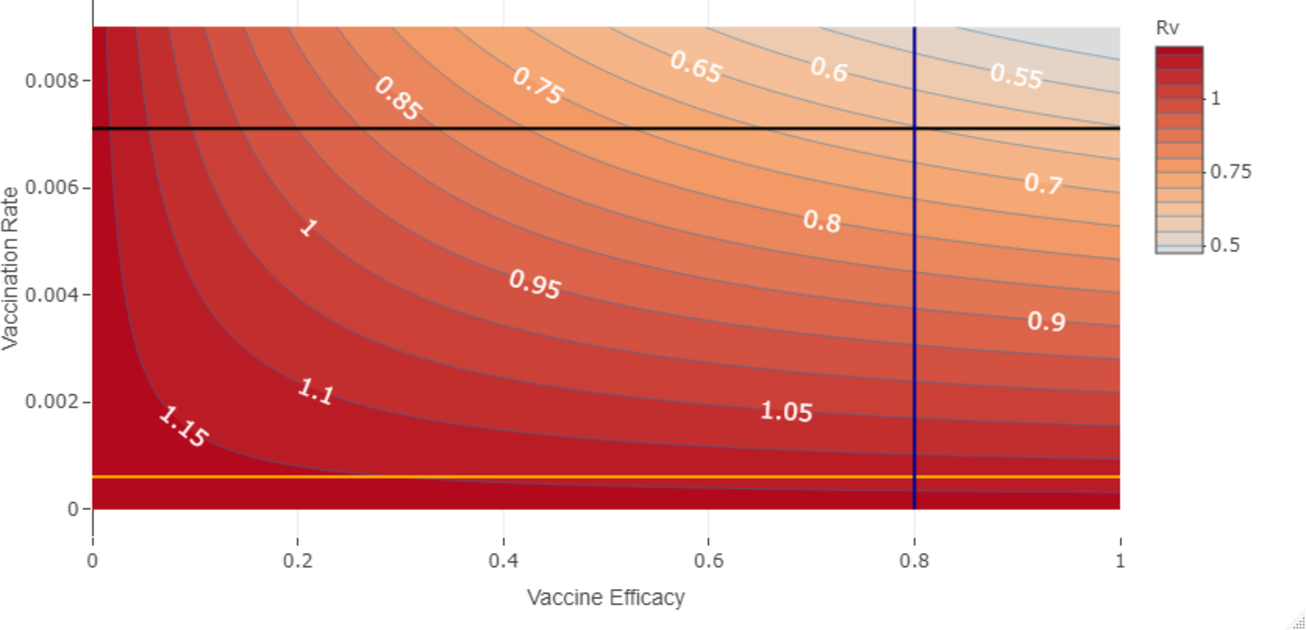
\includegraphics[scale=0.6, keepaspectratio]{Figures/Rv_contour}
    \caption{
    Contour plot  of $R_0^V$ as a function of $ \epsilon $ and $ \lambda_V $ and  
        vaccine-induced
        immunity average time of half year. orange line represents the 
        value of $\lambda_{Vbase}=\num{0.000611}$, corresponding to a coverage 
        $x_{coverage} = \num{0.2}$ and a horizon time $T=\num{365}$ days.
        Intersection of black line and blue line show a scenario in which it is
        possible to have the $R_V=0.65$, considering a vaccine efficacy of 
        \num{0.8} and a vaccination rate 
        of \num{0.7}.}
    \label{fig:rvcontour1}
\end{figure*}
<<<<<<< HEAD
%
\begin{figure*}[tbh]
    \centering
      \includegraphics[scale=0.7, keepaspectratio]{No-Lockdown-Vaccination.pdf}
    \caption{No lockdown Region $R_v<1$.
=======

\Cref{fig:rvcontour1} shows the efficacy of the vaccine
as a function of the vaccination rate. The blue line, $ \varepsilon = 0.8 $,
tells us what value of $ \lambda_V $ to take for which to have
the level curve where $ R_0^V<1 $.

\begin{figure*}[tbh]
    \centering
      \includegraphics[scale=0.7, keepaspectratio]{Figures/No-Lockdown-Vaccination}
    \caption{
        Vaccine efficacy versus vaccination rate feasibility.
        In the gray shaded region $R_V<1 $ and in the white region $ R_V >1 $. 
        Note that, for our scenario, we consider no lockdown individuals.
>>>>>>> origin/overleaf-2021-01-06-2308
    \href{https://plotly.com/~AdrianSalcedo/52/}{%
		https://plotly.com/~AdrianSalcedo/52/}
    }
    \label{fig:Nolockdown}
\end{figure*}
<<<<<<< HEAD
%
%
\begin{figure*}[tbh]
    \centering
      \includegraphics[scale=0.7, keepaspectratio]{Lockdown-Vaccination.pdf}
    \caption{lockdown Region $R_v<1$.
=======

In the gray region of the \cref{fig:Nolockdown}, you can see
the values of vaccine efficacy and vaccination rate for which
$R_0^V <1 $. In this figure, we consider that the lockdown effect is not present.
If we take $ \varepsilon = 0.2 $, we can see that we always have $ R_0^V> 1 $
with which choice of $ \lambda_V $.

\begin{figure*}[tbh]
    \centering
      \includegraphics[scale=0.56, keepaspectratio]{Figures/Lockdown-Vaccination}
    \caption{
        Vaccine efficacy versus vaccination rate feasibility.
        In the gray shaded region $R_V<1 $ and in the white region $ R_V >1 $. 
        Note that, for our scenario, we consider lockdown individuals.
>>>>>>> origin/overleaf-2021-01-06-2308
        \href{https://plotly.com/~AdrianSalcedo/54/}{%
		https://plotly.com/~AdrianSalcedo/54/}
    }
    \label{fig:Lockdown}
\end{figure*}
<<<<<<< HEAD
=======

In the\cref{fig:Lockdown}, we take into account that the lockdown effect is
present. We can see that the gray region, $ R_0 ^ V <1 $, is much larger than in
the figure. Note that we can choose smaller values for $ \varepsilon $ and $
\lambda_V $ when we do have an individual lockdown.
>>>>>>> origin/overleaf-2021-01-06-2308
